\documentclass[journal, letterpaper]{IEEEtran}
%\documentclass{scrartcl}

\usepackage[ngerman,english]{babel}
%\usepackage[latin1]{inputenc}
\usepackage[utf8]{inputenc}
\usepackage[T1]{fontenc}
\usepackage{amsmath}
\usepackage{amsthm}
\usepackage{amsfonts}
\usepackage{tikz}
\usepackage{verbatim}
\usepackage{subcaption}
\usepackage{algorithm}
\usepackage{algorithmic}
\usepackage[pdftex]{hyperref}

\renewcommand{\algorithmicrequire}{\textbf{Input:}}
\renewcommand{\algorithmiccomment}[1]{\ \ // #1} % C-like // Comments

\hyphenation{render}

% No clubs and widows allowed
\clubpenalty10000
\widowpenalty10000
\displaywidowpenalty=10000

\begin{document}

%\title{Simulating elastic spheres without external forces}
%\subtitle{Project 1 for class CS6491 Computer Graphics}
\title{Swirl \\
	{\large Project 2 for class CS6491 Computer Graphics}}
%\author{Sebastian Weiss}
\author{Sebastian Weiss, Kristian Eberhardson\\ \today}
%\date{\today}

\maketitle

\begin{tikzpicture}[remember picture,overlay]
   \node[anchor=north east,inner sep=0pt] at (current page.north east)
              {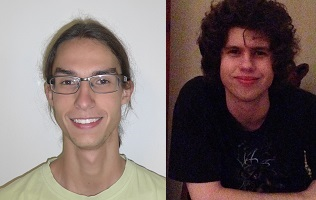
\includegraphics[scale=1]{pic}};
\end{tikzpicture}

\section{Objective}
We are provided with a starting and ending frame, called $A_0$ and $A_1$. We wish to create a continuous, affine and steady motion which interpolates $A_0$ and $A_1$.
 
\section{Input}
The Frames $A_0$ and $A_1$ consist of a point $P_i$ and a right hand coordinate system of orthogonal vectors $I_i$, $J_i$, and $K_i$, each of the same length ($i \in \{0,1\}$).
\subsection{Terms} 
1. An \underline{affine} transformation in three dimensions can be expressed as a 4x4 matrix multiplied onto a point or a vector, is reversible, and can be expressed solely as a combination of rotation, translation, and scaling.
\newline
2. A \underline{continuous} transformation is one in which $\forall \epsilon>0 \; \exists \delta>0 \; \text{s.th.} \; |P_x - P_y|<\epsilon \; \forall x,y \; \text{with} \; |x-y|<\delta$. $P_x$ and $P_y$ denotes the interpolated point at time $x$ and $y$. Intuitively, this means we can draw the motion with a pen in a single stroke.
\newline
3. A \underline{steady} transformation preserves the angle between a pair of frames, and is independent of some time t. 

\section{Related interpolation schemes}

\subsection{Logarithmic spiral in 2D}
A series of pairwise adjacent frames converge to a fixed point F when the motion is repeated indefinitely.  This motion preserves the angle between each frame, which we denote $\alpha$.  This motion also uses the same scaling factor between each pair of adjacent frames, so we calculate $m = (A_1).length / (A_0).length$.  Because we estimate curves as lines consisting of finitely many points in Processing, we can recursively follow the motion to F, and the program will terminate in a finite amount of time; this is the approach Professor Rossignac uses in his project: "Patterns of Similar Frames and Interpolation".  The steps are to rotate the current frame A by $\alpha$ scale by m, and then have the function call itself with the new frame's parameters.  This coincidentally gives us all the in-between keyframes as well, since we are using them to find F. 

\subsection{Linear interpolation in 3D}
For all points in $A_0$, draw a straight line to its corresponding point in $A_1$.  Motion is simply moving the frame along these lines.  This is neither an elegant solution nor does it preserve the area of the frame.

\subsection{Projected log spiral + Translation}


\section{Proposed model}
We wish to create a swirling motion in 3D related to the logarithmic spiral. Therefore, we are using a combination of linear rotation around the rotation axis $N$ with the origin in $F$ and an exponential scaling with the factor $m$. We propose the following formula:
\begin{equation}
 P(t) := F + m^t FP_0 ^{\;\circ} (\alpha t; N)
\label{eq:Interpolation}
\end{equation}

\subsection{3D rotation}
A rotation in 2D is very straightforward because there is no choice of the rotation axis. In 3D we're given the rotation axis and rotate around it in the following way:

\begin{equation}
\begin{array}{lcl}
 X^{\circ}(\alpha; N) &:=& W + U^{\circ}(\alpha; N) \\
                        & =& W + \cos \alpha U - \sin \alpha (N \times U) \\
 \multicolumn{3}{l}{\text{with } W := W\angle\underline{N} = (W\bullet\underline{N})\underline{N}} \\
 \multicolumn{3}{l}{\text{and } U = X-W}
\end{array}
\label{eq:Rotation}
\end{equation}

\subsection{Calculating $N$, $\alpha$ and $m$}
Since $m$ is the scaling factor, it is calculated as:
\begin{equation}
 m := |I_1| / |I_0|
\label{eq:m}
\end{equation}
Because $I_i$, $J_i$, and $K_i$ are of the same length for each $i$, it does not matter which we use. 
 
To calculate the rotation axis $N$, we first define 
\begin{equation}
\Delta I:= I_1 - I_0, \ \Delta J := J_1 - J_0, \ \Delta K := K_1 - K_0
\end{equation}
Then we pick the largest vector in the euclidean norm out of 
\begin{equation}
N_a := \Delta I \times \Delta J, \ N_b := \Delta I \times \Delta K, \ N_c := \Delta J \times \Delta K
\end{equation}
We call the largest vector $N$. Since $I_i$, $J_i$ and $K_i$ form an orthogonal basis, these vectors all point in the same direction and differ only in the scaling. The reasons for choosing the largest one are numerically issues. Some of these $N$'s can be very small when the rotation axis is almost parallel to the frame axes, they are zero if they are exactly parallel. The special case when all $N$'s are zero, so $\Delta I$, $\Delta J$ and $\Delta K$ are all zero, happens if there is no rotation at all. See section \ref{NoRot} on how to deal with this case. In the later computation, we always need the normalized vector $\underline{N}:=N/|N|$.
  
Furthermore, we need the rotation angle $\alpha$. To compute this angle, we first project each basis vector into the plane defined by $\underline{N}$ and normalize them:
\begin{equation}
\begin{array}{lcl}
 proj(X) &:=& X - X\angle\underline{N} = X - (X \bullet \underline{N})\underline{N} \\
 norm(X) &:=& X / |X| \\
 B' &:=& norm(proj(B_i)) \ \forall B \in \{I_0,...,K_1\}
\end{array}
\label{eq:ProjBasis}
\end{equation}
Then we define
\begin{equation}
 \alpha = \max \{ \cos^{-1}(I_0' \bullet I_1'), \cos^{-1}(J_0' \bullet J_1'), \cos^{-1}(K_0' \bullet K_1') \}
\label{eq:}
\end{equation}
We take the maximum angle here because all angles are equal by the definition of $N$. At most one of these angles can be zero, this happens in the case if the rotation axis is exactly orthogonal to that frame axis.

\subsection{Calculating $F$}
Now we have $N$, $\alpha$ and $m$ and we can compute $F$ now by solving the equation system
\begin{equation}
 P_1 = P(1) := F + m FP_0 ^{\;\circ} (\alpha; N)
\label{eq:Feq}
\end{equation}
This system is a linear system in the three variables $F_x$, $F_y$ and $F_z$. We obtain an explicit formulation for $F$ by converting it into matrix form, solving it using Cramer's Rule and applying simplification. For purposes of notation, we introduce the following variables for the vector components: $P_0=(P_{0,x},P_{0,y},P_{0,z})^T, P_1=(P_{1,x},P_{1,y},P_{1,z})^T,\\ \underline{N}=(N_x,N_y,N_z)^T$.
\begin{equation}
\begin{array}{lcl}
	F_x &=& (m P_{0,x} + m^3 P_{0,x} - P_{1,x} - m^2 P_{1,x} \\
		&& + m (1+m) (\cos\alpha - 1) (P_{0,x} - P_{1,x}) (N_x^2 + N_z^2) \\
		&& - m (1+m) (\cos\alpha - 1) (P_{0,y} - P_{1,y}) N_x N_y \\
		&& - m (1+m) (\cos\alpha - 1) (P_{0,z} - P_{1,z}) N_x N_z \\
		&& - m (m-1) \sin\alpha (P_{0,y} - P_{1,y}) N_z \\
		&& + m (m-1) \sin\alpha (P_{0,z} - P_{1,z}) N_y \\
		&& - 2 m^2 P_{0,x} \cos\alpha + 2 m P_{1,x} \cos\alpha ) \\
		&& / (m-1)(1 + m^2 - 2m\cos\alpha)
\end{array}
\end{equation}
\begin{equation}
\begin{array}{lcl}
 F_y &=& -(m^2 P_{0,y} - m^3 P_{0,y} + P_{1,y} - m P_{1,y} \\
		&& + m (1+m) (\cos\alpha - 1) (P_{0,x} - P_{1,x}) N_x N_y \\
		&& + m (1+m) (\cos\alpha - 1) (P_{0,y} - P_{1,y}) N_y^2 \\
		&& + m (1+m) (\cos\alpha - 1) (P_{0,z} - P_{1,z}) N_y N_z \\
		&& - m (m-1) \sin\alpha (P_{0,x} - P_{1,x}) N_z \\
		&& + m (m-1) \sin\alpha (P_{0,z} - P_{1,z}) N_x \\
		&& - m P_{0,y} \cos\alpha + m^2 P_{0,y} \cos\alpha \\
		&& - m P_{1,y} \cos\alpha + m^2 P_{1,y} \cos\alpha) \\
		&& / (m-1)(1 + m^2 - 2m\cos\alpha)
\end{array}
\label{eq:}
\end{equation}
\begin{equation}
\begin{array}{lcl}
 F_z &=& -(m^2 P_{0,z} - m^3 P_{0,z} + P_{1,z} - m P_{1,z} \\
		&& + m (1+m) (\cos\alpha - 1) (P_{0,x} - P_{1,x}) N_x N_z \\
		&& + m (1+m) (\cos\alpha - 1) (P_{0,y} - P_{1,y}) N_y N_z \\
		&& + m (1+m) (\cos\alpha - 1) (P_{0,z} - P_{1,z}) N_z^2 \\
		&& - m (m-1) \sin\alpha (P_{0,y} - P_{1,y}) N_x \\
		&& + m (m-1) \sin\alpha (P_{0,x} - P_{1,x}) N_y \\
		&& - m P_{0,z} \cos\alpha + m^2 P_{0,z} \cos\alpha \\
		&& - m P_{1,z} \cos\alpha + m^2 P_{1,z} \cos\alpha) \\
		&& / (m-1)(1 + m^2 - 2m\cos\alpha)
\end{array}
\label{eq:}
\end{equation}


\subsection{Dealing with special cases}
These are the cases in which there is either no fixed point or more than one around which our motion rotates steadily.

\subsubsection{No rotation}\label{NoRot}

\subsubsection{No rotation, no scaling}
(N = 0, have only translation)

\subsubsection{pure scaling}
For this case, we only need to calculate m.  Then, we can just scale the motion by m.

\section{Results}

\end{document}